11. \begin{figure}[ht!]
\center{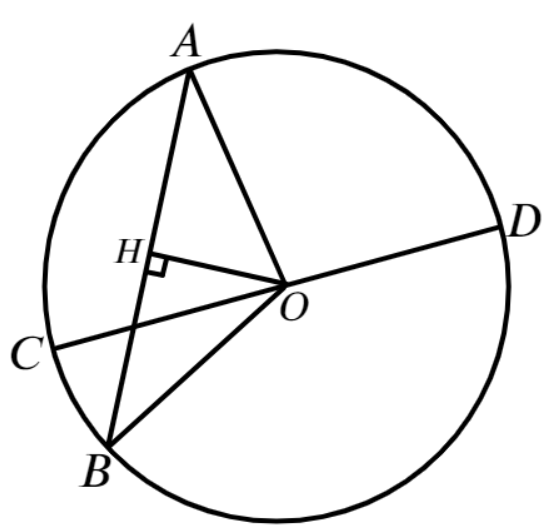
\includegraphics[scale=0.35]{g9-11.png}}
\end{figure}\\
В треугольнике $OAB$ стороны $OA$ и $OB$ равны, так как являются радиусами. Тогда он равнобедренный и $OH$ является не только высотой, но и медианой, а поэтому $OC=OB=\sqrt{OH^2+HB^2}=\sqrt{64+16}=4\sqrt{5}.$\newpage\noindent
